%%%%%%%%%%%%%%%%%%%%%%%%%%%%%%%%%%%%%%%%%%%%%%%%%%%%%%%%%%%%%%%
%
% Welcome to Overleaf --- just edit your LaTeX on the left,
% and we'll compile it for you on the right. If you open the
% 'Share' menu, you can invite other users to edit at the same
% time. See www.overleaf.com/learn for more info. Enjoy!
%
%%%%%%%%%%%%%%%%%%%%%%%%%%%%%%%%%%%%%%%%%%%%%%%%%%%%%%%%%%%%%%%
\documentclass[letterpaper,11pt]{article}

\usepackage{latexsym}
\usepackage[empty]{fullpage}
\usepackage{titlesec}
\usepackage{marvosym}
\usepackage[usenames,dvipsnames]{color}
\usepackage{verbatim}
\usepackage{enumitem}
\usepackage[hidelinks]{hyperref}
\usepackage{fancyhdr}
\usepackage[english]{babel}
\usepackage{tabularx}
\usepackage{fontawesome5}
\usepackage{multicol}
\usepackage{graphicx}
\setlength{\multicolsep}{-3.0pt}
\setlength{\columnsep}{-1pt}
\input{glyphtounicode}

%----------FONT OPTIONS----------
% sans-serif
% \usepackage[sfdefault]{FiraSans}
% \usepackage[sfdefault]{roboto}
% \usepackage[sfdefault]{noto-sans}
% \usepackage[default]{sourcesanspro}

% serif
% \usepackage{CormorantGaramond}
% \usepackage{charter}


\pagestyle{fancy}
\fancyhf{} % clear all header and footer fields
\fancyfoot{}
\renewcommand{\headrulewidth}{0pt}
\renewcommand{\footrulewidth}{0pt}

% Adjust margins
\addtolength{\oddsidemargin}{-0.6in}
\addtolength{\evensidemargin}{-0.5in}
\addtolength{\textwidth}{1.19in}
\addtolength{\topmargin}{-.7in}
\addtolength{\textheight}{1.4in}

\urlstyle{same}

\raggedbottom
\raggedright
\setlength{\tabcolsep}{0in}

% Sections formatting
\titleformat{\section}{
  \vspace{-4pt}\scshape\raggedright\large\bfseries
}{}{0em}{}[\color{black}\titlerule \vspace{-5pt}]

% Ensure that generate pdf is machine readable/ATS parsable
\pdfgentounicode=1

%-------------------------
% Custom commands
\newcommand{\resumeItem}[1]{
  \item\small{
    {#1 \vspace{-2pt}}
  }
}

\newcommand{\classesList}[4]{
    \item\small{
        {#1 #2 #3 #4 \vspace{-2pt}}
  }
}

\newcommand{\resumeSubheading}[4]{
  \vspace{-2pt}\item
    \begin{tabular*}{1.0\textwidth}[t]{l@{\extracolsep{\fill}}r}
      \textbf{#1} & \textbf{\small #2} \\
      \textit{\small#3} & \textit{\small #4} \\
    \end{tabular*}
}

\newcommand{\resumeSubSubheading}[2]{
    \item
    \begin{tabular*}{0.97\textwidth}{l@{\extracolsep{\fill}}r}
      \textit{\small#1} & \textit{\small #2} \\
    \end{tabular*}\vspace{-7pt}
}

\newcommand{\resumeProjectHeading}[2]{
    \item
    \begin{tabular*}{1.001\textwidth}{l@{\extracolsep{\fill}}r}
      \small#1 & \textbf{\small #2}\\
    \end{tabular*}\vspace{-7pt}
}

\newcommand{\resumeSubItem}[1]{\resumeItem{#1}\vspace{-4pt}}

\renewcommand\labelitemi{$\vcenter{\hbox{\tiny$\bullet$}}$}
\renewcommand\labelitemii{$\vcenter{\hbox{\tiny$\bullet$}}$}

\newcommand{\resumeSubHeadingListStart}{\begin{itemize}[leftmargin=0.0in, label={}]}
\newcommand{\resumeSubHeadingListEnd}{\end{itemize}}
\newcommand{\resumeItemListStart}{\begin{itemize}}
\newcommand{\resumeItemListEnd}{\end{itemize}}

%-------------------------------------------
%%%%%%  RESUME STARTS HERE  %%%%%%%%%%%%%%%%%%%%%%%%%%%%


\begin{document}

% %----------PROFILE PICTURE----------
% 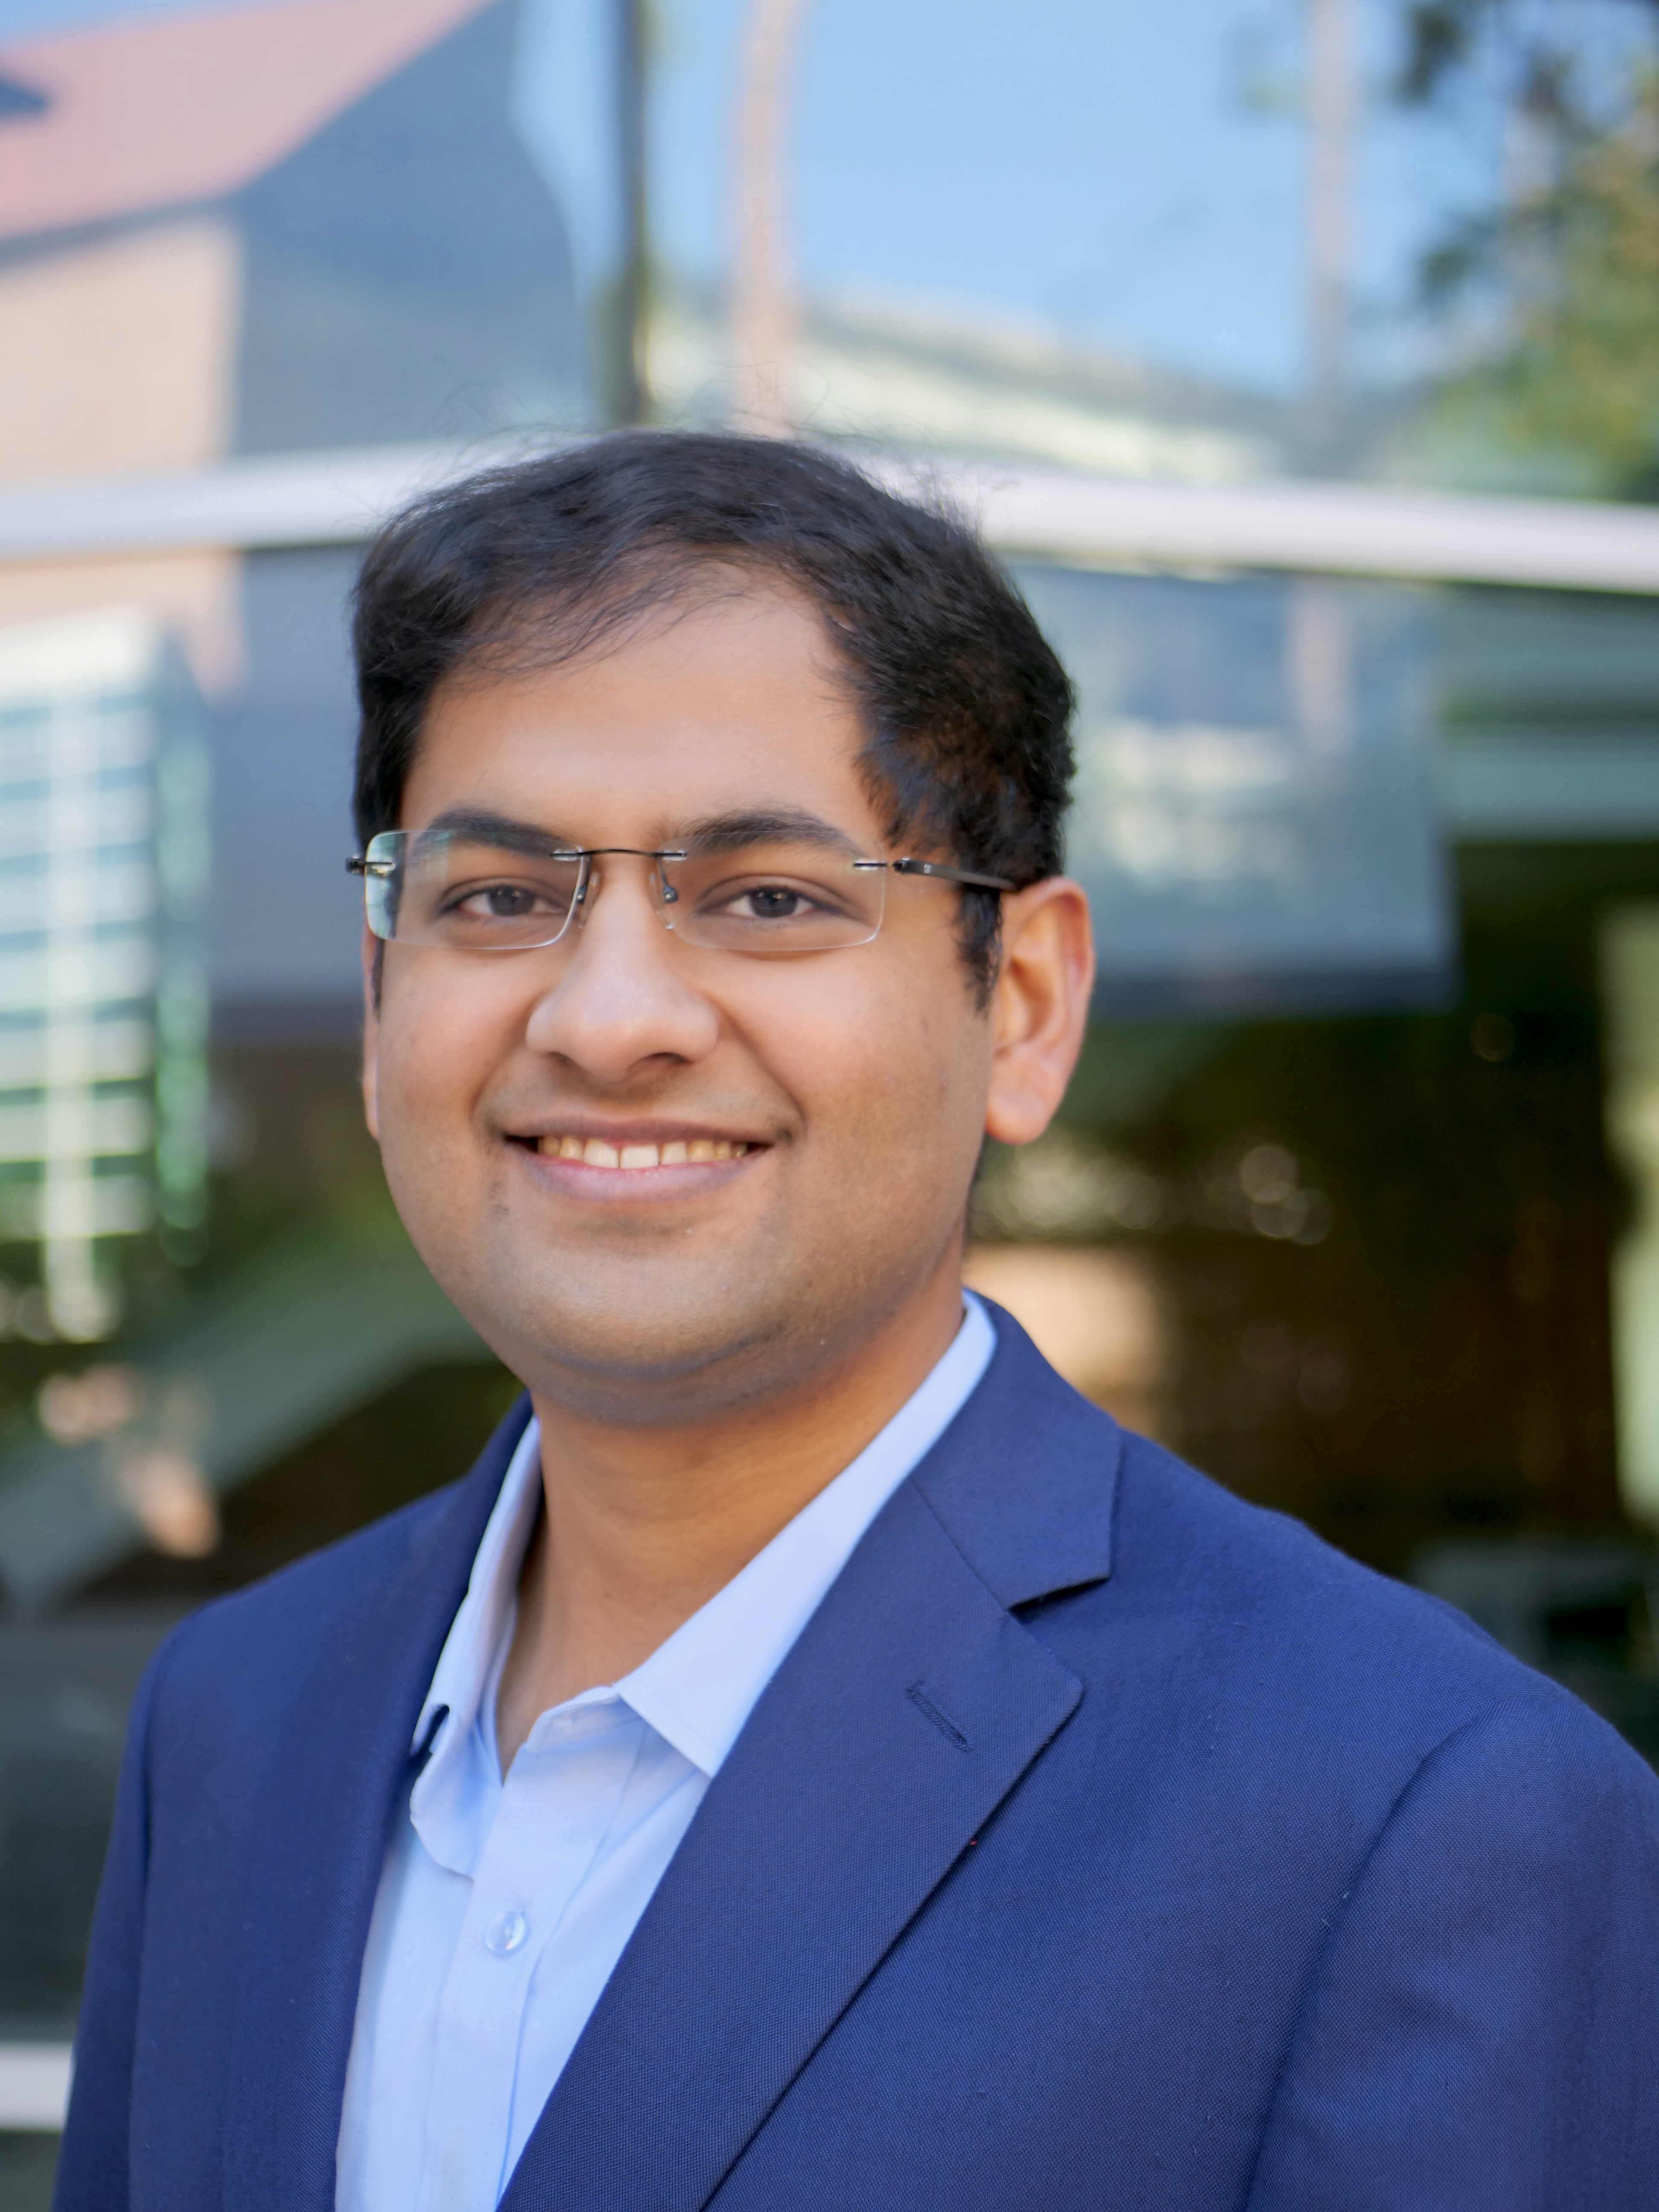
\includegraphics[width=0.1\linewidth]{P1040649.JPG}
% \quad \raisebox{2\height}{\Huge \scshape Aadit Kamat}\\
%----------HEADING----------
\begin{center}
\raisebox{2\height}{\Huge \scshape Aadit Kamat}  
\quad \faPhone\ +(1)352-709-5920 \quad ~ \href{mailto:aaditkmt@gmail.com}{\raisebox{-0.2\height}\faEnvelope\ \underline{aaditkmt@gmail.com}} ~ \quad 
    \href{https://github.com/aaditkamat}{\raisebox{-0.2\height}\faGithub\ \underline{github.com/aaditkamat}}
\end{center}

%-----------Objective-----------
\section{Objective}
Software engineer with experience in cloud-based backend systems, full-stack web development, and data-driven consulting. 
Skilled in AWS, Python, Node.js, and microservices architecture, with a passion for building scalable, secure, and user-focused solutions. 

%-----------EXPERIENCE-----------
\section{Experience}
  \resumeSubHeadingListStart
    \resumeSubheading
      {Visa Worldwide Pte Ltd}{March 2022 -- September 2022}
      {Software Engineer}{Singapore, SG}
      \resumeItemListStart
        \resumeItem{Developed and deployed Spring Boot-based microservices to support high-volume transaction processing (>100K TPS), aligning with cloud-native architecture and performance goals.}
        \resumeItem{Designed and integrated RESTful APIs with frontend components for internal admin portals, improving scalability and enabling multi-regional Innovation Centre operations across APAC and EMEA}
        \resumeItem{Developed unit tests to validate functional requirements and ensure WCAG accessibility compliance for the IC portal}
      \resumeItemListEnd

    \resumeSubheading
      {Shopee Singapore Pte Ltd}{May 2021 -- March 2022}
      {Quality Assurance \(QA\) Engineer}{Singapore, SG}
      \resumeItemListStart
        \resumeItem{Diagnosed and resolved complex technical issues in containerized environments, reducing test failures by 25 \% and significantly improving deployment stability}
        \resumeItem{Developed and maintained over 100 automated test cases for the promotion modules Shopee’s Android app  to enhance the experience for millions of users}
        \resumeItem{Led hands-on training for 50 engineers on Espresso and UiAutomator, cutting onboarding time and boosting automated test coverage by 15\%}
      \resumeItemListEnd

    \resumeSubheading
      {Atomionics Pte Ltd}{December 2020 -- March 2021}
      {Software Engineering Intern}{Singapore, SG}
      \resumeItemListStart
        \resumeItem{Collaborated with senior physicists specializing in cold atom physics to develop a desktop application using PyQt and QtDesigner for real-time experiment monitoring.}
        \resumeItem{Interfaced with M-Lab’s FPGA based control systems - Sinara and Kasli hardware - via ArtiQ to retrieve and visualize experimental data}
        \resumeItem{Built interactive dashboards featuring knobs and dials to ensure low latency tuning of TTL and DDS I/O signals and hardware synchronization, facilitating fine-grained control over quantum experiments}
      \resumeItemListEnd
      
    \resumeSubheading
      {NUS Information Technology}{December 2018 -- March 2019}
      {Test Automation Intern}{Singapore, SG}
      \resumeItemListStart
        \resumeItem{Designed and built a React.js web portal to streamline NUS IT’s annual firewall rule review process, replacing a manual, email-based workflow}
        \resumeItem{Integrated ADFS authentication with Passport.js OAuth to enable secure, department-based access}
        \resumeItem{Automated retrieval of firewall data on a nightly basis via Tufin APIs using cron jobs and stored them with MongoDB}
      \resumeItemListEnd
      
    \resumeSubheading
      {Autodesk Pte Ltd}{December 2018 -- March 2019}
      {Test Automation Intern}{Singapore, SG}
      \resumeItemListStart
        \resumeItem{Automated regression tests in Python, reducing manual regression testing effort by 90+ hours}
        \resumeItem{Performed cross-platform testing across multiple versions of Autodesk products using CI/CD pipelines with Jenkins to ensure consistency and stability}
        \resumeItem{Devised and implemented a merge plan to consolidate common functionalities across test codebases, improving maintainability and reducing duplication}
      \resumeItemListEnd
      
    \resumeSubheading
      {Learnseeker Pte Ltd}{December 2018 -- March 2019}
      {Software Engineering Intern}{Singapore, SG}
      \resumeItemListStart
        \resumeItem{Built an SMS Dashboard with Ruby on Rails to track and visualize metrics related to leads generated}
        \resumeItem{Developed a Marketing Dashboard to enable easier customer segmentation and campaign targeting}
        \resumeItem{Redesigned internal CRM software to better visualize customer retention metrics and drive data-informed decision making}
      \resumeItemListEnd
  \resumeSubHeadingListEnd

%-----------PROJECTS-----------
\section{Projects}
    \resumeSubHeadingListStart
        \resumeProjectHeading
          {\textbf{LegalLingo} $|$ \emph{Webpack, Node.js, Express.js, Typescript, Google Cloud}}{September 2024 - September 2024}
          \resumeItemListStart
            \resumeItem{Built LegalLingo, a Node.js-based Chrome extension that analyzes legal language (e.g., Terms of Service, Privacy Policies) for predatory or user-unfavorable clauses using Gemma 2.0 APIs within Google Cloud Vertex AI}
            \resumeItem{Addressed a critical gap for both non-native English speakers and general audiences unfamiliar with complex legal jargon, promoting digital transparency and user empowerment}
          \resumeItemListEnd
        \resumeProjectHeading
          {\textbf{DSSD LEAP Dashboard} $|$ \emph{React, Redux, D3.js, TailwindCSS}}{February 2025 - April 2025}
          \resumeItemListStart
            \resumeItem{Built an interactive web application with React and D3.js to track energy efficiency KPIs, enabling policy makers to assess LEAP program impact}
            \resumeItem{Deployed web application on Netlify so that stakeholders can easily access and showcase metrics}
          \resumeItemListEnd
       \resumeProjectHeading
          {\textbf{EchoChat} $|$ \emph{Expo Go, Typescript, Websockets, Mailgun, Firebase, Jest}}{September 2023 - December 2023 }
          \resumeItemListStart
            \resumeItem {Resolved critical TypeScript errors across the codebase, improving overall developer experience and reducing runtime issues in development environments}
            \resumeItem{Implemented email verification functionality using Mailgun to create secure onboarding flows}
          \resumeItemListEnd
        \resumeProjectHeading
          {\textbf{Jacksonville Energy Authority(JEA)} $|$ \emph{Excel, PowerBI}}{September 2024 - November 2024 }
          \resumeItemListStart
            \resumeItem{Created mockups based on Excel data tracking employee performance and customer satisfaction metrics}
            \resumeItem{Effectively translated business requirements into functional PowerBI dashboard designs for executive decision-making}
          \resumeItemListEnd 
    \resumeSubHeadingListEnd

%-----------PROGRAMMING SKILLS-----------
\section{Technical Skills}
\begin{itemize}[leftmargin=0.15in, label={}]
    \small{\item{
    \textbf{Programming Languages}{: Python, JavaScript, TypeScript, R, SQL, HTML, CSS} \\
    \textbf{Frameworks \& Libraries}{: React.js, Node.js, Express, Flask, PyQt, Qt Designer, Pandas, NumPy, Matplotlib, Seaborn, scikit-learn, Jupyter, Plotly} \\
    \textbf{DevOps \& Cloud Platforms}{:Docker, Nginx, Firebase, Heroku, Google Cloud Platform (Vertex AI, Cloud Functions), Git, GitHub}\\
    \textbf{Databases}{: MongoDB, PostgreSQL}\
    \textbf{Testing \& Automation}{: JUnit, Espresso, UiAutomator, PyTest, Selenium, Jenkins}\\
    \textbf{Data Science \& Analytics}{: Exploratory Data Analysis (EDA), Regression Analysis, Data Envelopment Analysis (DEA), Biostatistics, Predictive Modeling, PowerBI, Excel}\\
    \textbf{Healthcare \& Research Tools}{: Variant Effect Predictor (VEP), ArtiQ (Quantum Experiment Control), Tufin APIs (Firewall Data), NIH \& WHO Repositories, UF HiPerGator HPC Cluster}\\
    \textbf{Authentication \& APIs}{:OAuth 2.0, Passport.js, REST APIs, Gemma 2.0 APIs (LLM)} \\
    }}
\end{itemize}

%-----------EDUCATION-----------
\section{Education}
  \resumeSubHeadingListStart
    \resumeSubheading
      {University of Florida}{December 2024}
      {Master of Science in Information Systems and Operations Management}{Gainesville, FL}
    \resumeSubheading
      {National University of Singapore}{June 2021}
      {Bachelor of Computing in Computer Science}{Singapore, SG}
  \resumeSubHeadingListEnd
  
%

%-----------CERTIFICATIONS-----------
\section{Certifications}
   \resumeItemListStart
    \resumeItem{AWS Certified Cloud Practitioner, Jan 2025}
    \resumeItem{Databricks Fundamental Accreditation, Jan 2025}
    \resumeItem{End-to-End Data Engineering Project, Jun 2024}
   \resumeItemListEnd
\end{document}